\documentclass[11pt, oneside]{article}
\usepackage[utf8]{inputenc}
%\usepackage[czech]{babel}
\usepackage{a4wide}
\usepackage{graphicx}
\usepackage[textsize=footnotesize]{todonotes}
\usepackage{setspace}

%\usepackage[left=2.5cm,top=3cm,bottom=3cm,right=2.5cm]{geometry}
%\usepackage{arydshln} % dotted line
\usepackage{multirow} 
\usepackage{multicol}
\usepackage{color}
\usepackage{lmodern} % allows font size in millimeters

\usepackage{boxedminipage}
\usepackage{alltt}
\usepackage{amsmath}


\usepackage{url}

%uncomment for helvetica in headers
%\usepackage[scaled]{helvet}
%\renewcommand*\familydefault{\sfdefault}  %% Only if the base font of the document is to be sans serif


\usepackage{tabularx}
\usepackage{varwidth}


\usepackage{relsize}
\usepackage{hyperref}
\usepackage{graphics}


\usepackage{sectsty}
\usepackage{listings}
\usepackage{algorithm2e}

\providecommand{\SetAlgoLined}{\SetLine}
\providecommand{\DontPrintSemicolon}{\dontprintsemicolon}




\usepackage{listingsutf8}

% so that the PDF links link to the figure and not to its caption
\usepackage[hypcap]{caption}

\title{Automatic translation of movie subtitles}
\author{Karel Bílek, with substantial help by Jindřich Libovický}
%\date{} % Activate to display a given date or no date (if empty),
         % o


%%%%%%%%%%%%%%%%%%%%%%%%%%%%%%%
% Terminology
%%%%%%%%%%%%%%%%%%%%%%%%%%%%%%%


\newcommand{\subarrow}{-{}->}
\newcommand{\postgres}{Postgres}




\begin{document}
    \maketitle


\section{Introduction}
Follow the white rabbit.

\section{Building the Corpus}
\section{Initial data processing}

To ensure the full usability of the software from the very first moments when it is launched, some initial data is necessary.

\subsection{Retrieving data}

There are plenty of subtitle files in many languages available at the Internet these days, which can be easily downloaded.
However, it is problematic to download from most of the servers in bigger batches (thanks to anti-spam protection and so on); also, we wanted to avoid any copyright problems we would meet by using random subtitles from the internet. For this purpose, we asked the administrator of the biggest server providing the subtitles \emph{opensubtitles.org} for the data.

As a result of this we received all subtitle files in Czech and English from \emph{opensubtitles.org} with following licence condition (in Slovak):

\begin{quote}
\begin{verbatim}
Titulky mozem poskytnut, s tym ze:

- nebudu sa dalej sirit
- vsade, kde je to mozne a suvisi to s projektom, bude uvedena linka na
    www.opensubtitles.org (stranka programu, dokumentacia, program...)

Co sa tyka autorskych prav, tak neviem presne ako to je, ale myslim,
ze to je +- ok :)
\end{verbatim}
\end{quote}

\noindent with following English translation:

\begin{quote}
\begin{verbatim}
We can provide the subtitle files under following conditions:

- they won't be provided any further
- a link to www.opensubtitles.org will be placed whenever it's possible 
   (web page of the program, documentation, program itself...)

Considering the copyright law, I am not really sure how it is, 
but I think it's ok :)
\end{verbatim}
\end{quote}


\noindent We decided that this licence condition is acceptable for our purposes. 

As a matter of fact, the users of \emph{opensubtitles.org} agree with a statement where they declare they are holders of all rights to the content they post to the server, and provide the subtitle files as their own intellectual property for public use. Based on this and the licence, we think there are no more copyright issues.% Based on this statement we trust the users they really did what they declared.

%From this data we will create a parallel corpus of ...

\subsection{The data properties}

(In this section, we call \emph{subtitle} the whole subtitle file, \emph{chunk} is again the piece of text, displayed on screen at one time)

We received 3,076 MB of data in 139,538 files with a database index dump which did not exactly match the received content. After solving this problem we have 39,712 Czech subtitle files and 97,991 English files of 15,881 movies or TV shows episodes -- 3,032 MB of data.


Some subtitles are divide into more files, anyway 81\% of subtitles are in one piece. There is also just 1.7\% movies having subtitles only in multiple files. Moreover, we can assume that those which are in more parts, are probably just split the complete onces. To keep the chunk alignment simple we would delete those as well.

This caused that some movies lost its translation -- 64
of Czech and 218 of English. In total we will lost 3,5\% of movies. After this steps, the amount of data was 2,556 MB.

Because OpenSubtitles internally uses IMDB for adding information about movies and TV shows to subtitles, it was not hard to align subtitles of same movies and TV show episodes together, since all movie names used the same format (name and year), and the TV episodes were correctly marked.

However, this also caused one curious issue.
While looking more carefully at the data, we found there were 228 Czech subtitles files, 814 files in total having one particular movie ID and containing various content. This movie was Carmentica, a 21 seconds long silent film from 1884. This happened due to a server error at \emph{opensubtitles.org}, because the movie has ID {\tt tt0000001} at IMDB.

After doing all mentioned filtering we had 2,543 MB in 110,312 subtitle files (32,705 Czech, 77,607 English) of 15,552 movies / TV shows' episodes.

From these, the average subtitle file had XX chunks.

\subsection{Aligning the subtitles}

While we had enough metadata to align subtitles of the same movie together, there were still more than two subtitle files for each of the movies, so we needed to chose the best pair. Also, on these, we needed to align the actual chunks together. 

For elignment, we used two different approaches, which we then compared. TODO: COMPARISON. Damn, I am doing that today.

\subsubsection*{Editing distance}

While comparing two mostly identical subtitle files, there may appear some issues which cause that the timing of the files is not identical. There exist some cases where one chunk is split into more or two are merged into one. In both of this cases, two time declarations in the file remain the same and two time declarations are added or deleted. There are also a lot of subtitles for deaf people where from time to time some additional subtitle appears. 

From that we concluded that the best measure how subtitle files matches would be the editing distance of their time declarations since the cases mentioned above contributes relatively little to the score in contrast to some more significant mismatches. 
By that we mean taking all the time information (both the starts and the ends) as vectors, and then counting editing distance of those two vectors by dynamic algorithm.

As one of the papers (CITE!!!) proposed we used 0.6\,s as a tolerance for equality, not to be confused by slight differences in timing. Because the computation on whole files would be really time consuming, we limited it just for the first 100 time declarations in the files.

%when I rewrote it to scala it was actually much faster then in perl. Maybe we COULD do the whole files now :-)

The results were following: from 15,552 movies there was 22.2\,\%
with perfect matches and 3.1\,\% of total mismatches. The scores for partial matches are captured in table \ref{opensubtitles:matchTable}.

\begin{table}[h]

\begin{center}
\begin{tabular}{|c|c|}
\hline
amount of films & measure of match\\ \hline
22,2 \% & $= 100 \%$ match \\
45.7 \% & $\ge 90 \%$ match \\ 
56.2 \% & $\ge 80 \%$ match \\ 
63.0 \% & $\ge 70 \%$ match \\
69.2 \% & $\ge 60 \%$ match \\ \hline
\end{tabular}
\end{center}

\caption{Table capturing for how many movies there exist a matching pair of subtitle files with given measure of matching}\label{opensubtitles:matchTable}
\end{table}

%what does the "measure of match" mean in this context? I don't get it.

After looking at some randomly selected files we have decided to use just movies for which we have a pair of files with at least 70 \% match. Surprisingly, some worse scored pairs have quite high-quality translations, because they contain a lot of joined and split chunks, but generally, based on ran the quality of translation decreased with the match score.

On this files we run an aligning algorithm based just on the timing. The chunks were aligned if both the time of their start and time of their end differ less than by 0.6\ s. This gave us 884 MB of parallel data which consists of 13,636,022 chunks. In this we have 5,669,837 unique chunks, from which 3.7 \% appears more than once. On the other hand, chunks appearing more than once make 57.6 \% of the whole corpus.


\section{Training Machine Translation}
\label{chap:moses}

\todo{This whole chapter is VERY dense and VERY technical. I will have to rewrite it to something more readable..... MAYBE... DAMN THERE IS NO  TIME FOR ANYTHING}

Although our initial plan was to show translation memory only to the translator, we found out that we can also use the corpus to train a model for statistical machine translation. However, we also found that despite getting quite good results from the translation, the durations for getting the translations were too long, compared to the translation memory.

In this chapter, we will describe, how we trained the models, our results and how we managed to get the time cost down. The final model is a part of our project; the script to produce the model from the aligned data is not included, since it would require changes to EMS source code\footnote{EMS is the Experiment Management System, a system for managing Moses experiments, \url{http://www.statmt.org/moses/?n=FactoredTraining.EMS}}, which are untested at the moment and beyond the scope of this project.

Since we focus mainly on English to Czech translation, we modeled, trained and tested only for this way of translation. Training for the opposite way of translation would be possible, too, but all the necessary resources would double, while it would only benefit a small number of people.

This chapter requires some knowledge of phrase-based translation models and Moses in general. If you are not familiar with either, the short version of this chapter is that we are getting -- on subtitles -- better results with our machine translation than Google Translate, we are getting it fast, and we were able to fit it on a rather small virtual machine.


\section{Initial setup}
\subsection{Initial settings}

For training machine translation, we use our subtitle corpus, aligned by techniques described in Section~\ref{sec:aligning_subtitles}. Since we want to be more exact in this case, we used a more strict alignment, with 0.6\,s tolerance.

We do not require all the metadata about movie files for this task, so we added all the data together. We took away 15,000 sentences for MERT tuning (which proved to be too much) and 5,000 sentences for testing. The rest is training data.

Because of the way we took the testing sentences, they are all from different movies than the training data, except for at most one movie, that can have different sentences both in tuning and testing.

We run the standard EMS\footnote{EMS is the Experiment Management System, a system for managing Moses experiments, \url{http://www.statmt.org/moses/?n=FactoredTraining.EMS}} scenario on our data, which includes testing and counting BLEU score\footnote{BLEU is an automatic metric for measuring the success of a translation}. Although EMS counts both case-sensitive and case-insensitive BLEU, we chose the case-insensitive one.

We chose EMS instead of UFAL's own \texttt{eman}, simply for better documentation of the former and the inclusion of EMS in the standard Moses installation.

Initially, for the language model, we chose the IRSTLM\footnote{\url{http://hlt.fbk.eu/en/irstlm}} language model. For the translation model training, we used standard GIZA++.

We also measured the time for running the test translation.\footnote{This was achieved by adding time tracking code to the EMS source code; this code was submitted to Moses and actually ``survived'' in the main git repository for a few weeks, but was ultimately deleted, because it broke some edge cases.} Time was measured on a machine with Intel Core2 Quad CPU Q9550, with 4 cores with 2.83GHz, and 4GB of memory.

For reference on quality, we also translated the test set with Google Translate.

\begin{figure}[h]
\begin{center}
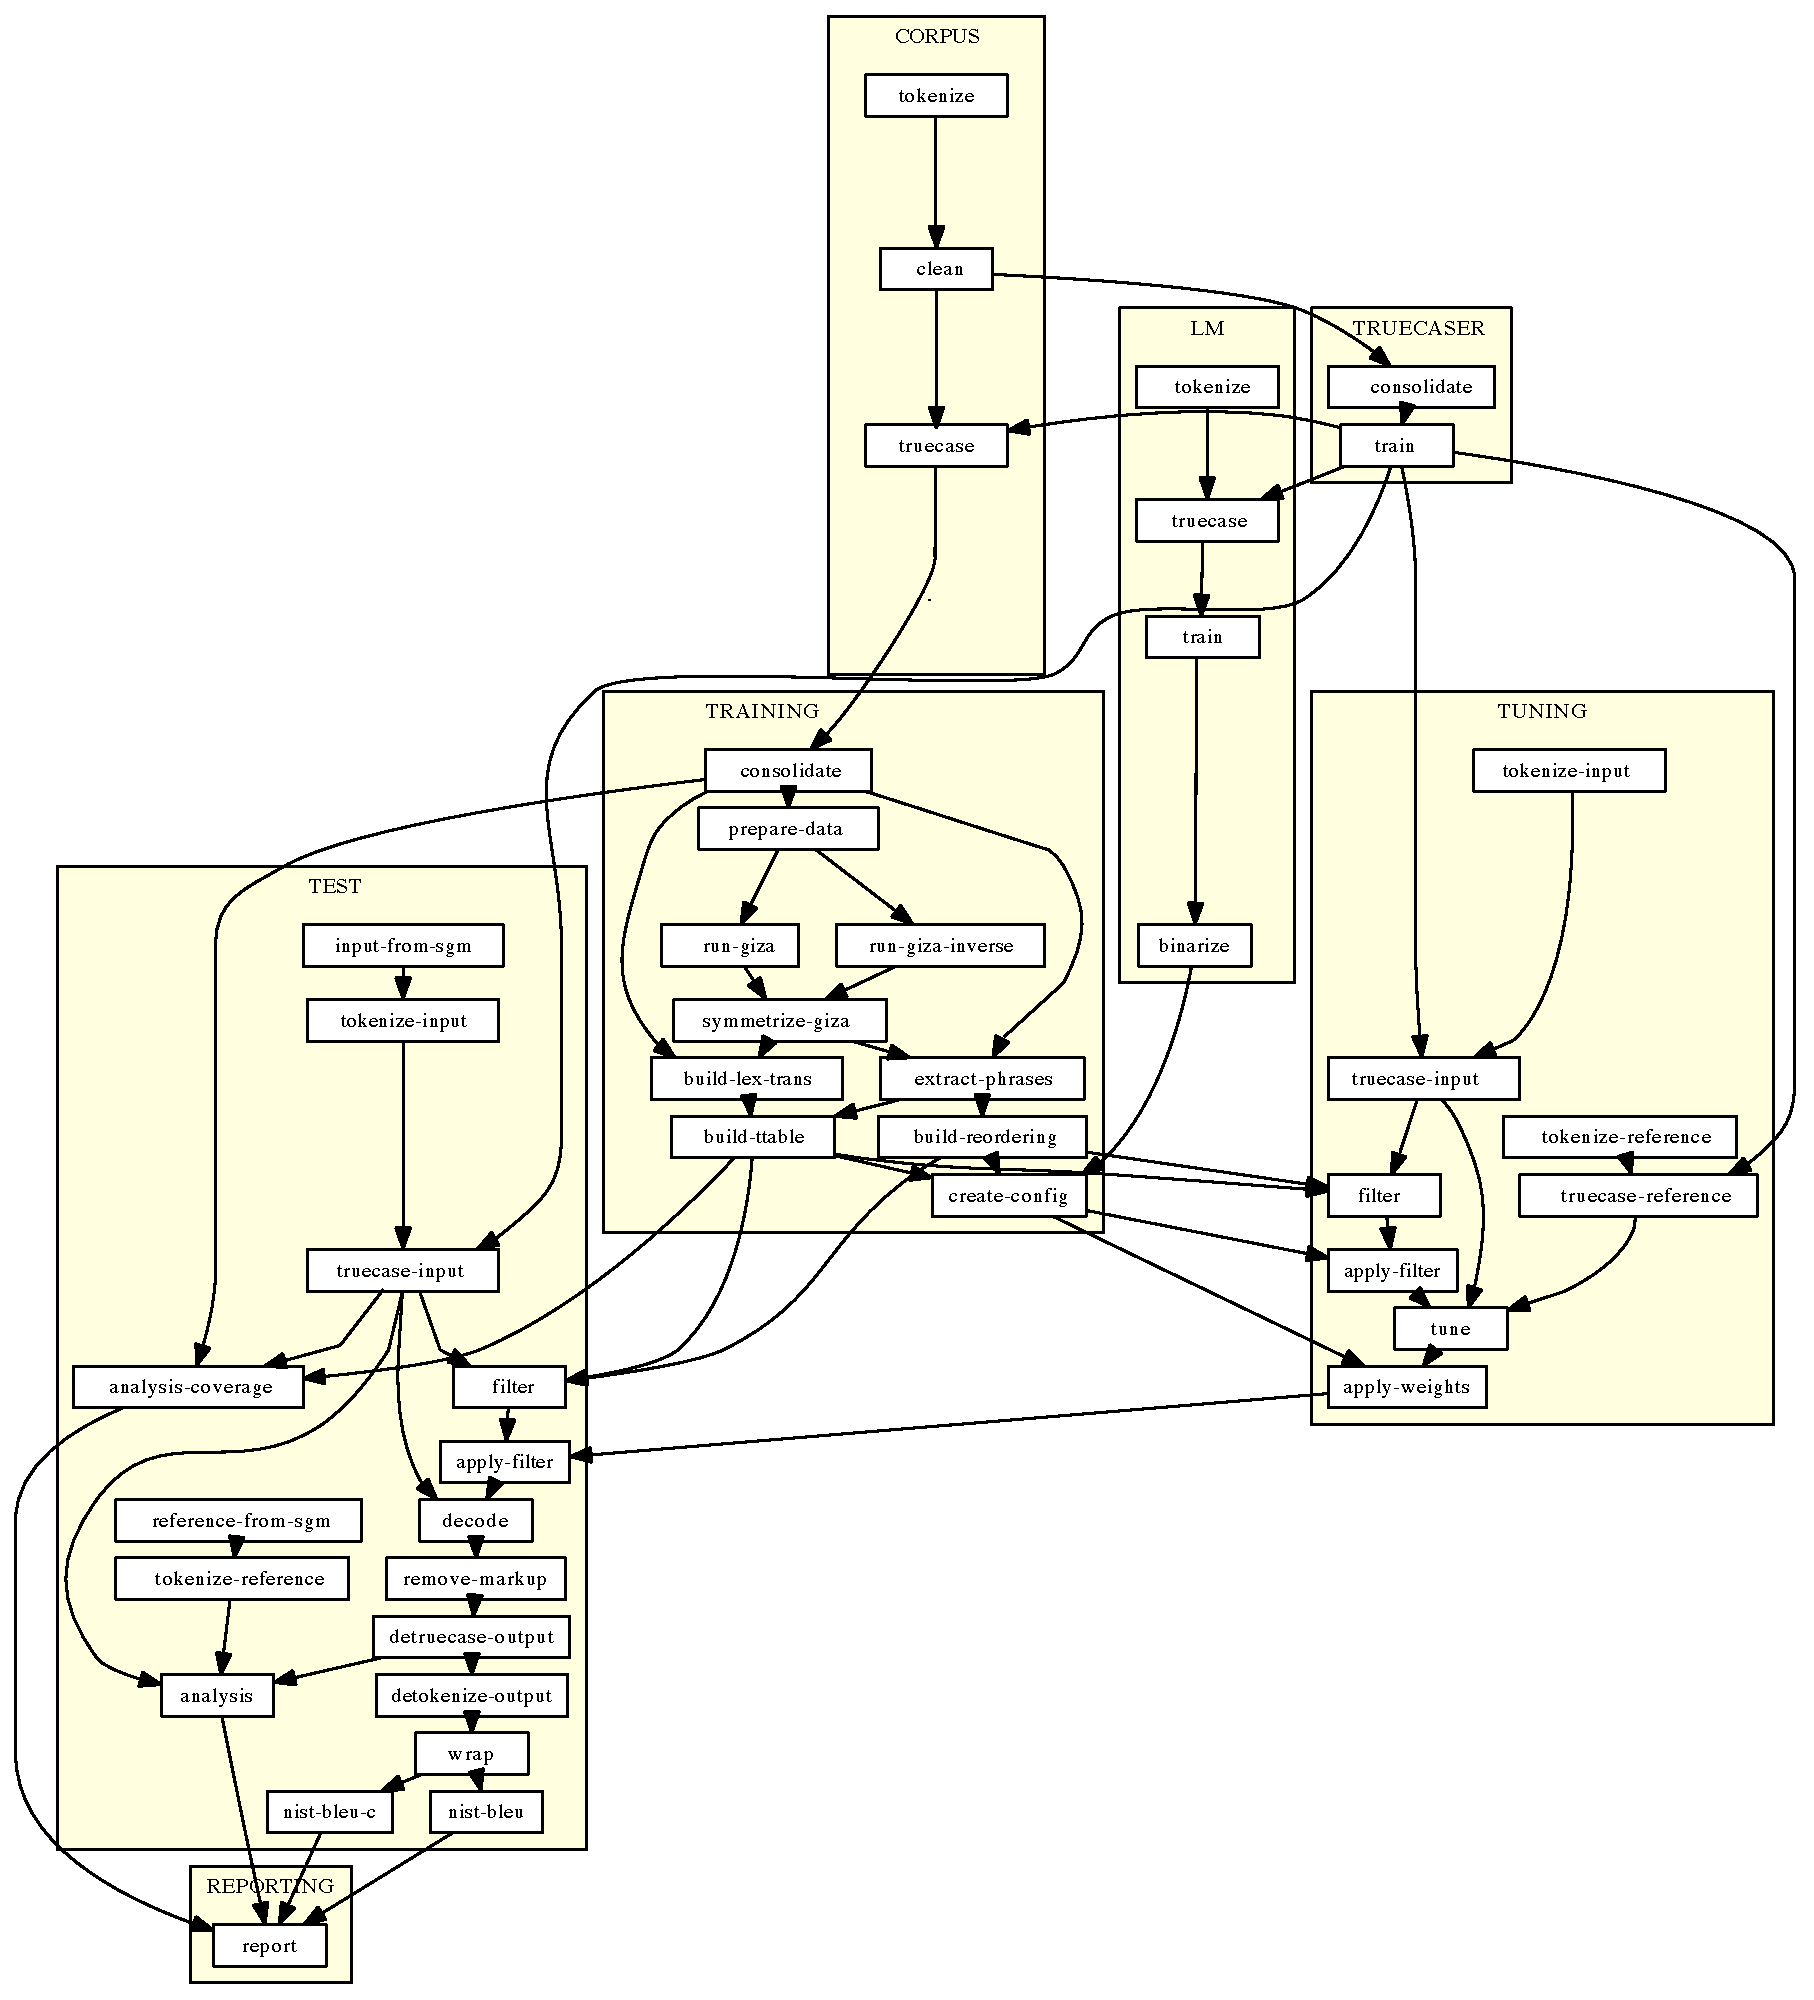
\includegraphics[width=0.8\textwidth]{figures/moses_13_graf.pdf}
\end{center}
\caption{Initial EMS set-up}\label{moses:initial}
\end{figure}

We can see the initial set-up in Figure~\ref{moses:initial}.
\subsection{Initial results}

The initial results are shown below.

\begin{table}[h]
\begin{center}
\begin{tabular}{|l|l|r|}
    \hline
    \textbf{Type} & \textbf{BLEU} & \textbf{incomplete average time per sentence} \\ \hline
    Initial setup & 23.88 & 147\,ms \\ \hline
    Google Translate & 19.07 & N/A \\  \hline
\end{tabular}
\end{center}

\caption{Initial results}\label{moses:initialresults}
\end{table}

We were very pleasantly surprised that our initial results were better than Google Translate, without really doing anything ``smart'' on our part. This is, however, definitely caused by a smaller domain. On the \texttt{newstest2012} set, Google's results were still quite good, while ours were terribly low\todo{I don't have time to show concrete numbers now. If I have more time, will do.}; the phrases in newspapers are completely different than phrases in subtitles.

The time looked good on the first glance; however, real times observed didn't line up with the results with the model. The difference was actually caused by EMT filtering (seen on \ref{moses:initial} as ``filter''). EMT, before doing the final tests, actually filters the models in such a way that only needed parts are loaded; the actual time of the final test is, then, much lower.

Also, even when we did not optimize for time spent on initial learning, the learning phase was too long to make any experiments effective. We addressed this issue, too.

\section{Changes in the set-up}
\subsection{Tuning set size}
The biggest issue with the training was actually the MERT tuning. If we cut down the number of phrases for MERT tuning, the time for tuning decreases significantly, while the BLEU doesn't decrease that much.
\begin{table}[h]
\begin{center}
\begin{tabular}{|l|l|r|}
    \hline
    \textbf{Tuning size} & \textbf{BLEU} & \textbf{Tuning time} \\ \hline
    15,000 & 23.88 & 12 hours 57 minutes \\ \hline
    1,000 & 22.95 & 16 minutes \\  \hline
\end{tabular}
\end{center}

\caption{Tuning set size decrease}\label{moses:initialresults}
\end{table}

\subsection{Turning off the filtering}
To know the real time of the translation, we needed to turn off the filtering in EMT, which required some slight modification in the source code. 

However, after that, we found out, that unfiltered models simply will not fit into the memory of the machine. Therefore, we had to both binarize the models and prune the phrase table.

\subsection{Pruning the phrase table}
Retrieving suitable elements from the translation table takes most of the time of the entire translation task. Therefore, making it smaller would make the translation task quicker.

As a first idea, we tried to prune the phrase table by using some factoring like short stems instead of full words. However, this showed up as a dead end; too short stems produce an absolutely empty phrase table, and longer stems do not shrink the phrase table significantly.

Instead, we tried another method, described in one of the papers\footnote{H. Johnson, J. Martin, G. Foster and R. Kuhn. (2007) \emph{Improving Translation Quality by Discarding Most of the Phrasetable}. In Proceedings of the 2007 Joint Conference on Empirical Methods in Natural Language Processing and Computational Natural Language Learning (EMNLP-CoNLL), pp. 967-975.}. It prunes the table using statistical signifance test, called Fisher's exact test\footnote{\url{http://en.wikipedia.org/wiki/Fisher's_exact_test}}. 

This method is implemented in Moses in \texttt{sigtest-filter} script; however, EMS doesn't support it in the main Moses repo. We had to add support for it to EMS, only to find out afterwards that Aleš Tamchyna from ÚFAL has already did that.

As described in the original paper, pruning the table actually did increase the BLEU score; what we lost by decreasing the tuning size, we got back by doing the pruning.

\begin{table}[h]
\begin{center}
\begin{tabular}{|l|l|r|}
    \hline
    \textbf{Pruning} & \textbf{BLEU} & \textbf{ttable size (gunzipped)} \\ \hline
    No & 22.59 & 2.10 GB \\ \hline
    Yes & 23.26 & 598MB \\  \hline
\end{tabular}
\end{center}

\caption{Pruning the phrase table}\label{moses:tablepruning}
\end{table}

\subsection{Binarizing the models}
All models -- reordering model, language model and translation table (both pruned and upruned) -- can be binarized. Binarization is a process in which the table is written in such a format that can be read from disk and loaded to memory only on-demand.

Loading from disk is slower than reading from memory, so binarizing is not helping us making the translation go quicker. However, it is helping us in fitting the models into memory at all.

\todo{table I guess}

\subsection{Smaller cube pruning}
\todo{this, find out what that is actually about}

Decreasing the cube pruning stack size also increases the time performance.

\section{Final remarks}
There is no spoon.


\end{document}
